% !TEX program = xelatex
\documentclass{article}
% include some packages
\usepackage{graphicx}
\usepackage{amsmath, amsfonts, amssymb}
\usepackage{tikz}
\usepackage[UTF8]{ctex}
\usepackage{hyperref}
\usepackage{dirtree}
\usepackage{listings}
\usepackage{xcolor}

% Path for my images
\graphicspath{{./images/}}
% infos about the doc
\begin{document}
\title{HW1: Neural Networks Report}
\author{王昊文}

\maketitle
% settings for code blocks
\definecolor{codegreen}{rgb}{0,0.6,0}
\definecolor{codegray}{rgb}{0.5,0.5,0.5}
\definecolor{codepurple}{rgb}{0.58,0,0.82}
\definecolor{backcolour}{rgb}{0.95,0.95,0.92}

\lstdefinestyle{mystyle}{
    backgroundcolor=\color{backcolour},   
    commentstyle=\color{codegreen},
    keywordstyle=\color{magenta},
    numberstyle=\tiny\color{codegray},
    stringstyle=\color{codepurple},
    basicstyle=\ttfamily\footnotesize,
    breakatwhitespace=false,         
    breaklines=true,                 
    captionpos=b,                    
    keepspaces=true,                 
    numbers=left,                    
    numbersep=5pt,                  
    showspaces=false,                
    showstringspaces=false,
    showtabs=false,                  
    tabsize=2
}

\lstset{style=mystyle}

% Change settings for caption
\renewcommand{\figurename}{Figure}

% Settings for the flow chart
\usetikzlibrary{shapes.geometric, arrows}
\tikzstyle{io} = [rectangle, rounded corners, minimum width=3cm, minimum height=1cm,text centered, draw=black, fill=red!30]
\tikzstyle{arrow} = [thick,->,>=stealth]
\tikzstyle{process} = [rectangle, minimum width=3cm, minimum height=1cm, text centered, draw=black, fill=orange!30]

% Document starts here
\section{Overview}
    The whole homework strictly follows the object-orientated philosophy, which 
    treats \emph{datatset}, \emph{data loader}, \emph{trainer}, \emph{logger} as 
    different objects, so that it can be very convinient to write your own custom
    objects. You can combine all your settings and put them under \verb|config.json|
    inside the root folder. \\ 
    \indent Also, you will find that the structure is highly similar to 
    \href{https://github.com/victoresque/pytorch-template}{pytorch template},
    but actually without any Pytorch! This gives me the chance to implement 
    a basic neural netork from scratch, and writing base classes. \\
    \indent In this homework, I will be using the \textbf{MNIST} dataset with mini-batch
    SGD.
    
\section{Details}
    \subsection{Data}
        In the MNIST dataset, we have a total of 60000 of training data, and 
        10000 testing data. We use a train:val split of 7:3, which indicates we 
        are going to have 42000 training samples and 18000 validation samples.
        This data is about classifying hand-written digits.
        Each input feature is $28 \times 28 = 784$ dimension. Since we are
        not using convolution, we will reshape the input features as $784 \times 1$ for convinience.
        The train:test ratio can be modified inside the \verb|config.json| 
        file under the root file. \\
        \indent Since we are using cross-entropy loss(configured inside json.config)
        , we have to one-hot encode the labels. Since the dataset contains ten-digit, 
        the lables will be one-hot encoded into a vector of shape $(10 \times 1)$,
        with the true lable be 1, and others be 0.\\
        \indent All features will be normalized by a factor of 255, so that the
        weights will not be affected by a super large value. Note, the reading
        of dataset is handled be the \emph{MNIST dataset} class and the preprocessing
        and spliting by the \emph{MNIST data loader} class.

    \subsection{Architecture}
        The model architecture is shown in figure \ref{fig:1}. Note that is defined
        under \verb|model.py|.         
        \begin{figure}
            \begin{tikzpicture}[node distance=1.9cm]
                \node (in1) [io] {Input layer};
                \node (pro1) [process, below of=in1, align=center] {FC1\\ $W: 300 \times 784$ \\ $b:300 \times 1$};
                \node (pro2) [process, below of=pro1] {ReLU};
                \node (pro3) [process, below of=pro2, align=center] {FC2\\ $W: 10 \times 300$ \\ $b:10 \times 1$};
                \node (pro4) [process, below of=pro3] {Softmax};
                \node (o1) [io, below of=pro4] {Output layer};
                \node (pro5) [process, right of=o1, xshift=3cm]{Cross-entropy};
                \node (o2) [io, right of=pro5, xshift=3cm] {Loss};
                \draw [arrow] (in1) -- node[anchor=east]{$y_0$} node[anchor=west]{$784 \times 1$} (pro1);
                \draw [arrow] (pro1) -- node[anchor=east]{$y_1$} node[anchor=west]{$300 \times 1$}(pro2);
                \draw [arrow] (pro2) -- node[anchor=east]{$y_2$} node[anchor=west]{$300 \times 1$}(pro3);
                \draw [arrow] (pro3) -- node[anchor=east]{$y_3$} node[anchor=west]{$10 \times 1$}(pro4);
                \draw [arrow] (pro4) -- node[anchor=east]{$y$} node[anchor=west]{$10 \times 1$}(o1);
                \draw [arrow] (o1) -- (pro5);
                \draw [arrow] (pro5) -- (o2);
            \end{tikzpicture}
            \caption{Architecture of our model} \label{fig:1}.
        \end{figure}
    \subsection{Implementation of Feed Forward and Back propogation}
        Below are some details of implementaion:
        \begin{lstlisting}[language=python, caption=feed forward]
    import numpy as np
    def forward(self, x):
        # Input layer
        self.tensors['y0'] = x
        # Input layer -> fc1
        self.tensors['y1'] = np.matmul(self.fc1['W'], self.tensors['y0']) + self.fc1['b']
        # ReLU layer
        self.tensors['y2'] = F.relu(self.tensors['y1'])
        # Output Layer
        self.tensors['y3'] = np.matmul(self.fc2['W'], self.tensors['y2']) + self.fc2['b']
        # Output layer
        self.tensors['y'] = F.softmax(self.tensors['y3'])
        # return classified results
        return self.tensors['y']
        \end{lstlisting}
        The above code will match figure \ref{fig:1}.
        \begin{lstlisting}[language=python, caption=back propogation]
    def backward(self, L_bp, m_batch):
        """
           Implement back prop process and compute the gradients
           :m_batch: mini batch size
           :L_bp: Backward pass of the loss
           :return: gradients
        """
        gradients = {}
        # The upstream gradient from the loss with softmax loss
        d_y = L_bp
        # Calculate the local gradients and multiply with upstream gradient
        gradients['dW2'] = (1. / m_batch) * np.matmul(d_y, self.tensors['y2'].T)
        gradients['db2'] = (1. / m_batch) * np.sum(d_y, axis=1, keepdims=True)
        # Calculate gradient of ReLU
        d_y2 = np.matmul(self.fc2['W'].T, d_y)
        d_y1 = np.multiply(d_y2, np.where(self.tensors['y1'] <= 0, 0, 1))
        gradients['dW1'] =  (1. / m_batch) * np.matmul(d_y1, self.tensors['y0'].T)
        gradients['db1'] =  (1. / m_batch) * np.sum(d_y1, axis=1, keepdims=True)
        return gradients
        \end{lstlisting}
        \verb|L_bp| is the back propogation value from the cross-entropy loss.
        Note that when softmax and cross-entropy combined, the backward pass 
        is only the true-class label, which is the one-hot encoded vector, mimus
        the predicted softmax score. \\
        \indent All the gradients are calculated by multiplying the upstream 
        gradient and the local gradient. Here we list out the local gradients.
        \begin{enumerate}
            \item $\frac{\partial}{\partial{W}} (Wx +b) = x^{\intercal}$
            \item $\frac{\partial}{\partial{b}} (Wx +b)$ \\
                The resulting derivative will be a column vector with all ones
                in it. Assume the matrix $Wx$ has shape $j \times k$, then the 
                vector should be $k \times 1$. Hence if we calculate the upstream 
                gradient times the local gradient, it would be equivalent of 
                summing over the rows of the upstream gradient.
            \item $\frac{\partial{L}}{\partial{o_i}} = p_i - y_i$ \\
                Where L is the cross-entropy loss, $o_i$ is the hidden layer value
                before the softmax activation, $p_i$ is the predicted score of 
                the softmax activation, and $y_i$ is the true label's score for
                class $i$, that is 1 for true class and 0 for negative.
            \item $\frac{\partial}{\partial{x_i}}\max{(0, x_i)}$
                \[
                    = 
                    \begin{cases}
                        0, \; \text{if} \; x_i < 0 \\
                        1, \; \text{if} \; x_i > 0
                    \end{cases}
                \]
        \end{enumerate}
    \subsection{Training and validation}
            As shown in figure \ref{fig:2} and \ref{fig:3}, we can see the change
            in loss and accuracy for training and validation at the training
            stage, when training with 100 epochs using SGD with a mini-batch size
            of 128. We can see from the accuracy graph that the training accuracy
            increases, while the validation accuracy flattens near 98\%. 
            This suggests that our model starts to overfit after 40 epochs, as 
            we might not get an accuracy over 98\% at the testing stage. This 
            hypothesis can be proved at the testing stage.
    \begin{figure}[h]
        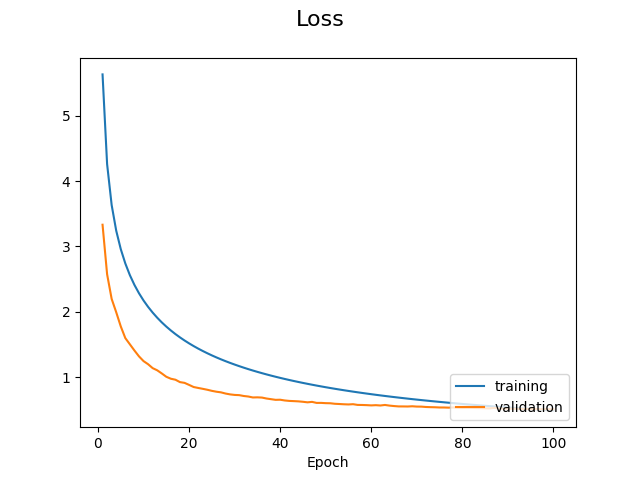
\includegraphics[scale=0.7]{Loss.png}
        \caption{Loss curve, Training v.s. Validation} \label{fig:2}
    \end{figure}
    \begin{figure}[h]
        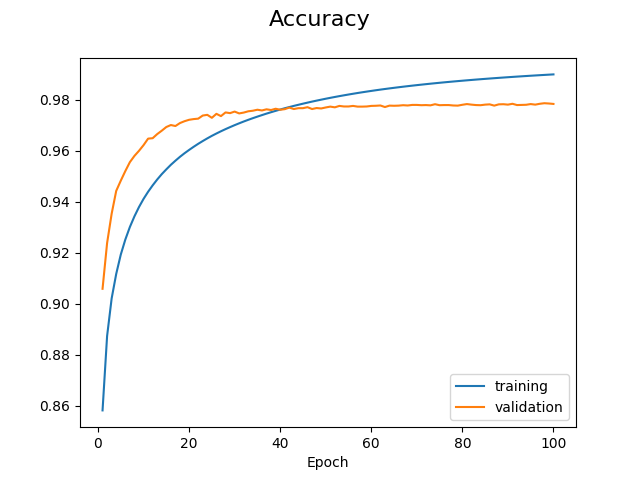
\includegraphics[scale=0.7]{Accuracy.png}
        \caption{Accuracy curve, Training v.s. Validation} \label{fig:3}
    \end{figure}
    \subsection{Performace}
        I have provided a best model \verb|best.npz| and the config 
        \verb|config.json| under the root folder.  To run \verb|test.py|, type 
        \verb|python test.py -c config.json -r best.npz| and run. As suggested 
        in the previous section, You should get approximately 97\% - 98\% of 
        testing accuracy.

\section{Short questions}

    \subsection{Deep neural network v.s. accuracy}
        If we use a very deep NN with a large number of neurons, will the accuracy
        increase? Well, sure, the \emph{training accuracy} will increase, since the 
        variance is getting larger as we get deeper(under the assumption that
        we are using activations for every fully-connected layers). However,
        it does not guarantee better \emph{testing accuracy}, as it might be 
        just overfitting to the distribution of the training data. We must 
        monitor the bias-variance trade-off in order to gain better performance, 
        not just by increasing the variance of the model.

    \subsection{Why validation?}
        Why do we need to valudate our model? If we don't validate our model, 
        then there is no other way to check for overfitting at the training stage.
        Note that we are \textbf{not allowed} to use the testing data
        while training. 
\section{Bonus: t-SNE results}
    \begin{figure}
        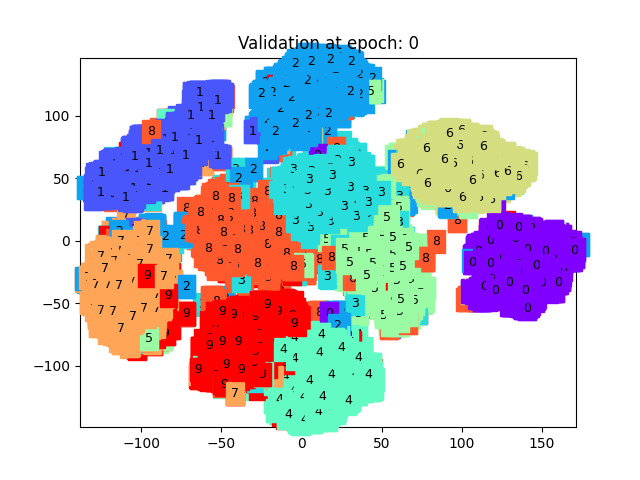
\includegraphics[scale=0.6]{Validation at epoch: 0.png}
        \centering
        \caption{t-SNE visualization of validation data at epoch 0} \label{fig:4}
    \end{figure}
    \begin{figure}
        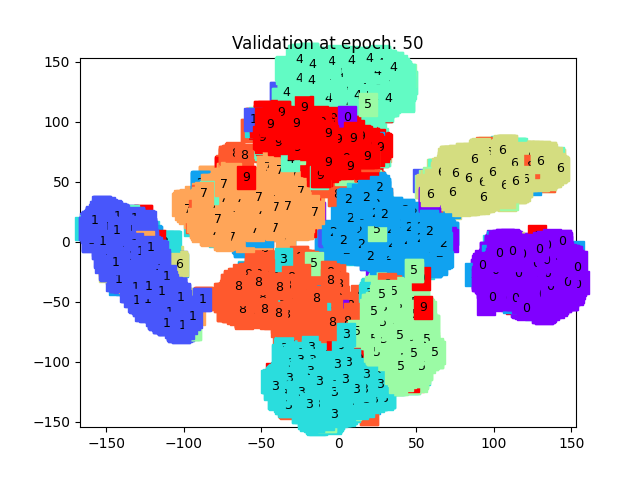
\includegraphics[scale=0.6]{Validation at epoch: 50.png}
        \centering
        \caption{t-SNE visualization of validation data at epoch 50} \label{fig:5}
    \end{figure}
    \begin{figure}
        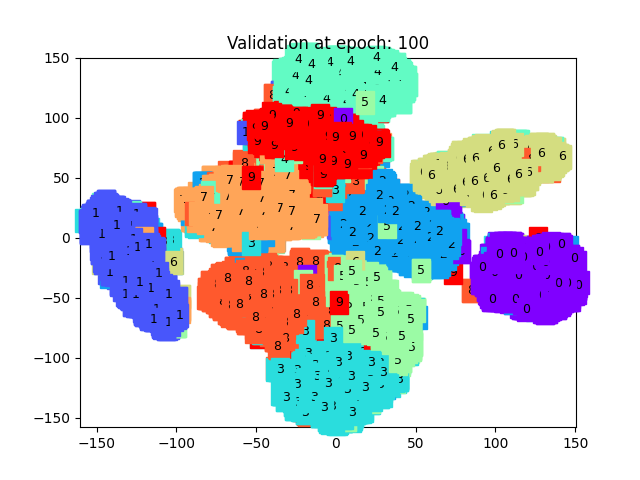
\includegraphics[scale=0.6]{Validation at epoch: 100.png}
        \centering
        \caption{t-SNE visualization of validation data at epoch 100} \label{fig:6}
    \end{figure}
    \begin{figure}
        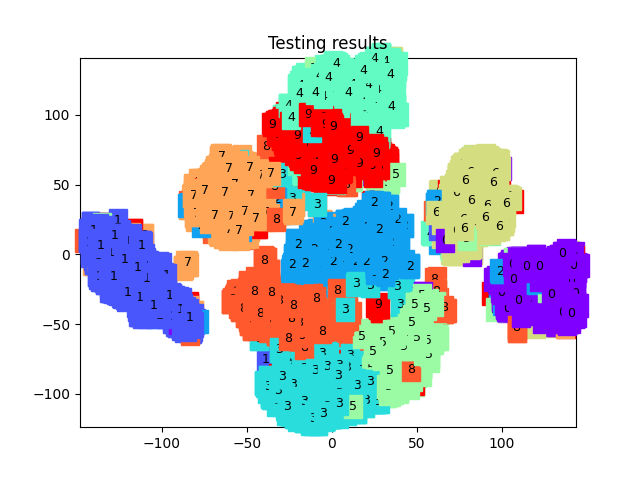
\includegraphics[scale=0.6]{Testing results.png}
        \centering
        \caption{t-SNE visualization of testing data} \label{fig:7}
    \end{figure}
    Figure \ref{fig:4}, \ref{fig:5}, \ref{fig:6} shows the t-SNE results on our
    data on the validation stage, during different epochs. Figure \ref{fig:7}
    shows the t-SNE results on the testing data. \\
    Since the visualization process consumes a lot of time, I commented this part out from my 
    code, and hence sklearn is not required to run my code.
\end{document}
